\chapter{一种容错性加强的自动缓存清理方法}\label{chap:clean}

\section{内存管理模块分析}

Spark框架由Scala语言编写。Scala语言是一种运行在JVM(Java Virtual Machine)的函数式编程语言。函数式编程语言相比于C++、Java等命令式编程语言的优点是将数据进行了分类,分为可变数据数据variable和不可变数据value。同时也提供了非常适合并行编程的函数式编程接口。函数式语言的这种特点就让它天然适用于分布式并行大数据处理领域。Scala语言还有一个独特的优势就是它是运行在JVM之上的,这就让Scala语言可以运行在所有支持JVM的平台上,这就使得Scala具有非常好的跨平台特性。但是对于Spark框架来说,他有完全独立的内存管理模块BlockManager。BlockManager也是运行在JVM上的一个进程。

\begin{figure}
    \centering
    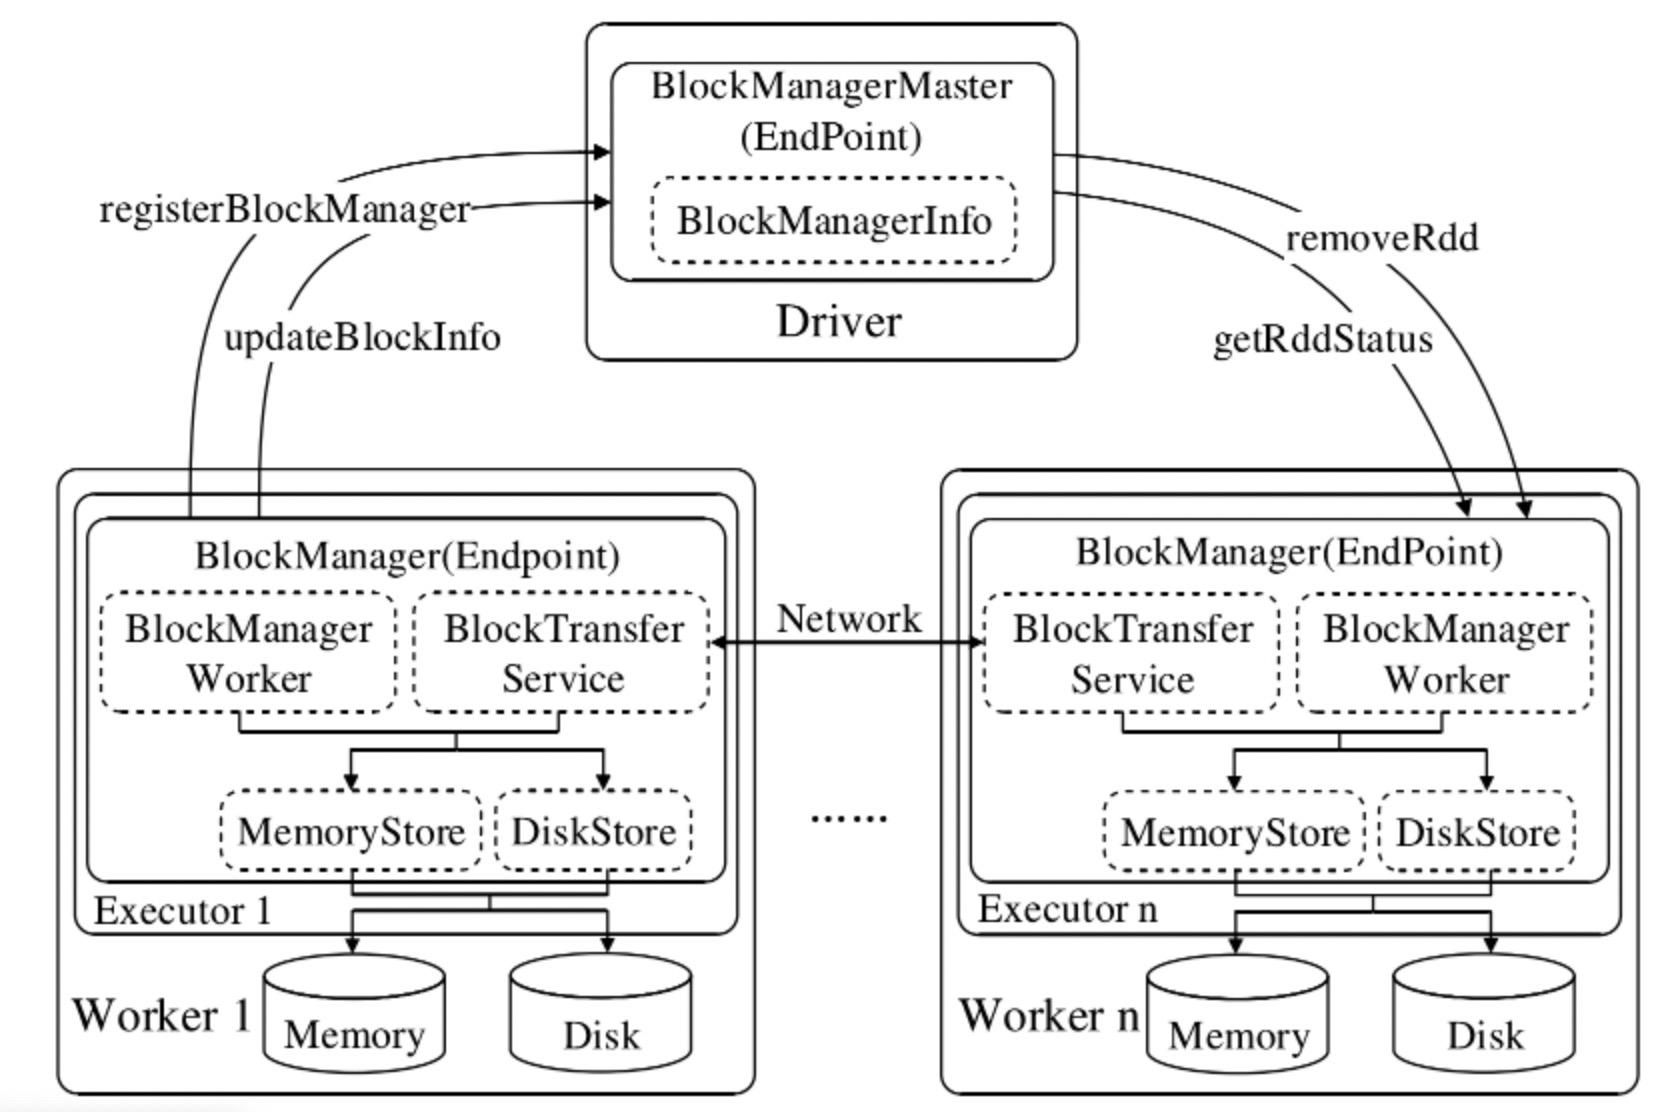
\includegraphics[width=0.99\textwidth]{Img/block-manager.jpg}
    \caption{BlockManager结构图}
    \label{fig:block-manager}
\end{figure}

\subsection{内存管理模块潜在问题}

BlockManager和JVM都有管理内存的功能,但是两者完全隔离,这就会有潜在的问题。BlockManager内存管理的原理非常简单。用户提交Spark应用的时候会通过配置文件指定Executor使用的内存总量,之后框架会向JVM申请内存创建Executor以及内部的BlockManager。BlockManager初始化之后会开始管理Executor整个内存空间。BlockManager向外提供了非常简单的接口,Get接口和Put接口。Get接口的参数为RDD数据的ID,如果数据存储在磁盘或者内存之中BlockManager就会返回具体的地址。Put接口的参数是RDD的应用和存储级别,比如MEMORY_ONLY、DISK_ONLY等,BlcokManager会根据存储级别将数据存储在不同位置。

框架的内存模型如图\ref{fig:memory-model}所示。Spark框架内存模型分为以下几个部分:Storage区域,Execution区域,Other区域。Other区域主要用于用户程序定义的数据结构。Execution内存用于框架执行,比如计算RDD的分区时数据就全部存储在Execution区域。Execution区域的内存有一个特点就是会主动地回收内存。他使用的方法是类似与引用计数的算法。比如一个图\ref{fig:simpl-dag}所示的简单的三个节点的计算图。计算得到数据B的时候B的数据就存储在Execution区域。因为计算C还会使用数据B所以数据B并不会立刻被替换出去。但是A会被立刻删除。在以后计算E的时候又会使用到数据A,但是数据A早已被删除,这就会造成数据丢弃,框架会通过容错算法重新计算数据A。

\begin{figure}
    \centering
    \includegraphics[width=0.99\textwidth]{}
    \caption{简单计算图 ####}
    \label{fig:simpl-dag}
\end{figure}

\begin{figure}
    \centering
    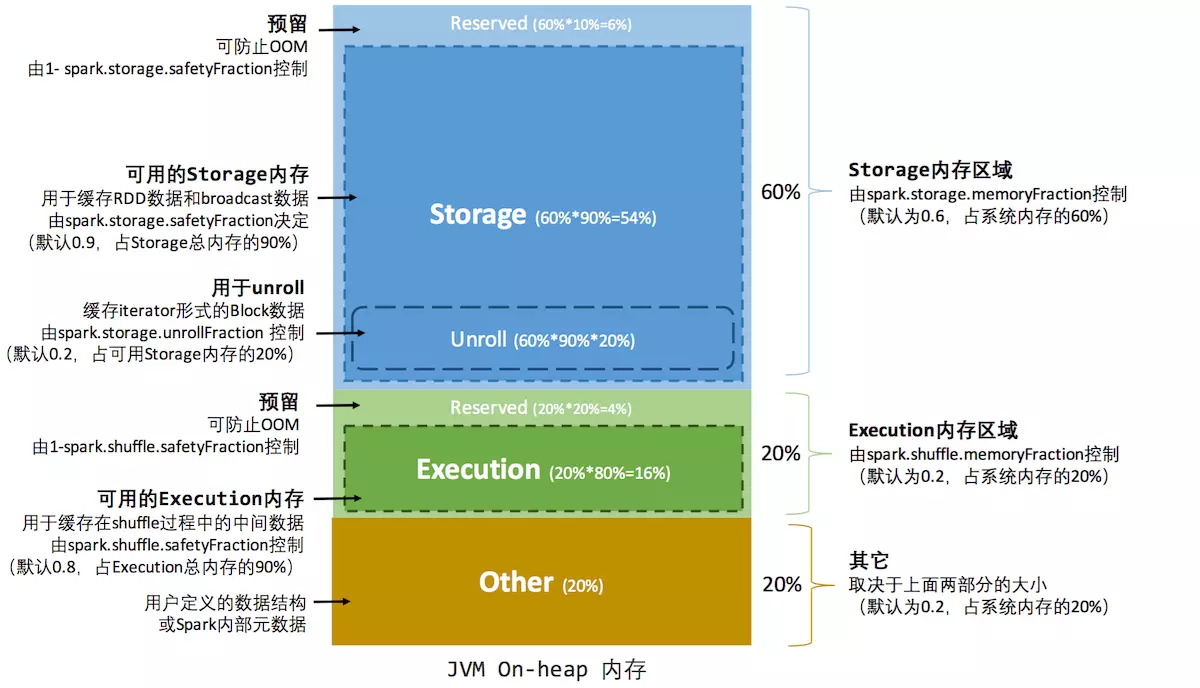
\includegraphics[width=0.99\textwidth]{Img/memory-model.png}
    \caption{内存模型}
    \label{fig:memory-model}
\end{figure}

对于内存管理来说是BlockManager内部的MemoryStore负责的。MemoryStore内部简单地通过一个整数变量记录Executor节点空闲的内存,当收到缓存请求时,MemoryStore会比较空闲空间和需要缓存的数据大小,如果空闲空间大于缓存数据就会保存缓存数据的引用在LinkedHashMap中,这样就能够避免数据被清理。

